\documentclass[12pt, titlepage]{article}

\usepackage{fullpage}
\usepackage[round]{natbib}
\usepackage{multirow}
\usepackage{booktabs}
\usepackage{tabularx}
\usepackage{graphicx}
\usepackage{float}
\usepackage{hyperref}
\hypersetup{
    colorlinks,
    citecolor=black,
    filecolor=black,
    linkcolor=red,
    urlcolor=blue
}
\usepackage[round]{natbib}

\newcounter{acnum}
\newcommand{\actheacnum}{AC\theacnum}
\newcommand{\acref}[1]{AC\ref{#1}}

\newcounter{ucnum}
\newcommand{\uctheucnum}{UC\theucnum}
\newcommand{\uref}[1]{UC\ref{#1}}

\newcounter{mnum}
\newcommand{\mthemnum}{M\themnum}
\newcommand{\mref}[1]{M\ref{#1}}

\title{SE 3XA3: Software Requirements Specification\\Title of Project}

\author{Team \#, Team Name
		\\ Kristine Uchendu (uchenduc)
		\\ Jason Nam (namy2)
		\\ Rylan Sykes (sykesr)
}

\date{\today}

% \input{../../Comments}

\begin{document}

\maketitle

\pagenumbering{roman}
\tableofcontents
\listoftables
\listoffigures

\begin{table}[bp]
\caption{\bf Revision History}
\begin{tabularx}{\textwidth}{p{3cm}p{2cm}X}
\toprule {\bf Date} & {\bf Version} & {\bf Notes}\\
\midrule
March 18, 2022 & 0 & Revision 0\\
\bottomrule
\end{tabularx}
\end{table}

\newpage

\pagenumbering{arabic}

\section{Introduction}

A key part of the development process is documentation of the modular breakdown of the system. The modular breakdown is exactly what it sounds like — the breaking down of our system (the Sketchy Super Mario Bros game) into individual modules that each hold one secret. This document will be outlining the system’s existing modules, what secret they are hiding as well as how they are designed for change. In the Anticipated and Unlikely Changes section, described will be changes foreseen in the design of the system as well as changes that appear to be unlikely for the system. In the following sections, the module structure will be discussed along with how they make up the system. Finally, there should be visual aids throughout the document with one of them being a table mapping how the system’s requirements and anticipated changes are met by the systems modules.

\section{Anticipated and Unlikely Changes} \label{SecChange}

This section lists possible changes to the system. According to the likeliness
of the change, the possible changes are classified into two
categories. Anticipated changes are listed in Section \ref{SecAchange}, and
unlikely changes are listed in Section \ref{SecUchange}.

\subsection{Anticipated Changes} \label{SecAchange}

Anticipated changes are changes that are foreseen in the design process of the system. These changes greatly factor into how the system is decomposed into modules, because the system is decomposed such that these changes are easier to make down the line. Essentially, each change described here should result in the modification of a singular model, should it actually be implemented. This is the design for change approach.


\begin{description}
\item[\refstepcounter{acnum} \actheacnum \label{ac1}:] The addition of new power up items for Mario to interact with.
\item[\refstepcounter{acnum} \actheacnum \label{ac2}:] The addition of new levels, and worlds (groupings of levels with the final challenge at the end.
\item[\refstepcounter{acnum} \actheacnum \label{ac3}:] The addition of more moving actors (antagonists for Mario to interact with in the game).
\item[\refstepcounter{acnum} \actheacnum \label{ac4}:] Changing the behaviours of existing modelled objects in the game.
\item[\refstepcounter{acnum} \actheacnum \label{ac5}:] The addition of new audio files for sound effects
\item[\refstepcounter{acnum} \actheacnum \label{ac6}:] Updates may be made to the graphics/animations of the characters.
\item[\refstepcounter{acnum} \actheacnum \label{ac7}:] The creation of a starting page for the game as well as the creation of end of game pages.

\end{description}

\subsection{Unlikely Changes} \label{SecUchange}

The module design should be as general as possible. However, a general system is
more complex. Sometimes this complexity is not necessary. Fixing some design
decisions at the system architecture stage can simplify the software design. If
these decision should later need to be changed, then many parts of the design
will potentially need to be modified. Hence, it is not intended that these
decisions will be changed.

\begin{description}
\item[\refstepcounter{ucnum} \uctheucnum \label{ucIO}:] Input/Output devices
\item[\refstepcounter{ucnum} \uctheucnum \label{ucInput}:] There will always be
  a source of input data external to the software.
\item [\refstepcounter{ucnum} \uctheucnum \label{ucSoftware}:] The number of players playing one game together (it will likely remain a single player game).

\end{description}

\section{Module Hierarchy} \label{SecMH}

This section provides an overview of the module design. Modules are summarized
in a hierarchy decomposed by secrets in Table \ref{TblMH}. The modules listed
below, which are leaves in the hierarchy tree, are the modules that will
actually be implemented.

\begin{description}
\item [\refstepcounter{mnum} \mthemnum \label{m1}:] Gradle Configuration Module
\item [\refstepcounter{mnum} \mthemnum \label{m2}:] Launcher Module
\item [\refstepcounter{mnum} \mthemnum \label{m3}:] Audio Module
\item [\refstepcounter{mnum} \mthemnum \label{m4}:] Actions Module
\item [\refstepcounter{mnum} \mthemnum \label{m5}:] Input Module
\item [\refstepcounter{mnum} \mthemnum \label{m6}:] Models Module
\end{description}


\begin{table}[h!]
\centering
\begin{tabular}{p{0.3\textwidth} p{0.6\textwidth}}
\toprule
\textbf{Level 1} & \textbf{Level 2}\\
\midrule

{Hardware-Hiding Module}
& \textbf{M5:} Input Module\\
\midrule

\multirow{2}{0.3\textwidth}{Behaviour-Hiding Module}
& \textbf{M3:} Audio Module\\
& \textbf{M4:} Actions Module\\
& \textbf{M6:} Models Module\\
\midrule

\multirow{1}{0.3\textwidth}{Software Decision Module}
& \textbf{M1:} Gradle Configuration Module\\
& \textbf{M2:} Launcher Module\\
\bottomrule

\end{tabular}
\caption{Module Hierarchy}
\label{TblMH}
\end{table}

\section{Connection Between Requirements and Design} \label{SecConnection}

The design of the system is intended to satisfy the requirements developed in
the SRS. In this stage, the system is decomposed into modules. The connection
between requirements and modules is listed in Table \ref{TblRT}.

There are many design decisions that need to be made to realize requirements for this system. The design of the system must make it easy to use and access. The user must be able to execute the system without failure, and perform actions with ease and simplicity. The Gradle configuration module and the launcher module of the system will be designed so that the game is accessible with simple configuration of the system. This will be able to fulfill FR1, NF8, and NF9. The design of the system must also allow user to perform all basic command of actions to Mario within the system. Mario must be able to appropriately move right, left, and up given a input by the user. The input must be delivered by a keyboard input. The design must accept appropriate input, whether that be left, right, or up. The design must not accept any other input that has no correlation within the system. This design decision will meet FR3, FR4, FR6, and NF10. The design must perform all interaction between models properly. One case could be when Mario interacts with a mushroom. Mario must become big Mario. Another case might involve a goomba interacting with Mario. Mario must die or big Mario must shrink if touched by a goomba. These interactions between models must be included in design decisions.

\section{Module Decomposition} \label{SecMD}

Modules are decomposed according to the principle of ``information hiding''
proposed by \citet{ParnasEtAl1984}. The \emph{Secrets} field in a module
decomposition is a brief statement of the design decision hidden by the
module. The \emph{Services} field specifies \emph{what} the module will do
without documenting \emph{how} to do it. For each module, a suggestion for the
implementing software is given under the \emph{Implemented By} title. If the
entry is \emph{OS}, this means that the module is provided by the operating
system or by standard programming language libraries.  Also indicate if the
module will be implemented specifically for the software.

Only the leaf modules in the
hierarchy have to be implemented. If a dash (\emph{--}) is shown, this means
that the module is not a leaf and will not have to be implemented. Whether or
not this module is implemented depends on the programming language
selected.

\subsection{Hardware Hiding Modules}

\subsubsection{Input Module (\mref{m5})}
\begin{description}
\item[Secrets:]The data structures and algorithms used for the keyboard and mouse inputs to interface with the software.
\item[Services:]Serves as an interface between the keyboard \& mouse and system
\item[Implemented By:] Mouse \& Keyboard
\end{description}

\subsection{Behaviour-Hiding Module}

\subsubsection{Audio Module (\mref{m3})}
\begin{description}
\item[Secrets:] The algorithms used to transmit the data stored in the audio files to be played through the users speakers.
\item[Services:] Acts as an API between the programmer and the hardware to programatically play sounds and music
\item[Implemented By:] libGDX
\end{description}

\subsubsection{Actions Module (\mref{m4})}
\begin{description}
\item[Secrets:] The behaviour of all actors in the game, including the behaviour of when the user sends an input to control Mario.
\item[Services:] Acts as a communication layer between the keyboard \& mouse input and the libGDX actor actions
\item[Implemented By:] N/A
\end{description}

\subsubsection{Models Module (\mref{m5})}
\begin{description}
\item[Secrets:] The data structures and algorithms used to store and manipulate the state of each actor in the game
\item[Services:] Allows the actors to exist in a game world and communicate with other actors
\item[Implemented By:] N/A
\end{description}

\subsection{Software Decision Module}

\subsubsection{Gradle Configuration Module (\mref{m1})}
\begin{description}
\item[Secrets:] The configurations used to define how Gradle will interact with the system
\item[Services:] Allows Gradle to interface with the game making it possible to install and update package necessary to execute the game.
\item[Implemented By:] Gradle
\end{description}

\subsubsection{Launcher Module (\mref{m2})}
\begin{description}
\item[Secrets:] The data structures used to instantiate the game
\item[Services:] Allows the user to launch the game
\item[Implemented By:] N/A
\end{description}


\section{Traceability Matrix} \label{SecTM}

This section shows two traceability matrices: between the modules and the
requirements and between the modules and the anticipated changes.

% the table should use mref, the requirements should be named, use something
% like fref
\begin{table}[H]
\centering
\begin{tabular}{p{0.2\textwidth} p{0.6\textwidth}}
\toprule
\textbf{Req.} & \textbf{Modules}\\
\midrule
FR1 & \mref{m1}, \mref{m2}\\
FR2 & \mref{m1}, \mref{m2}, \mref{m5}\\
FR3 & \mref{m4}, \mref{m5}\\
FR4 & \mref{m4}, \mref{m5}\\
FR5 & \mref{m4}, \mref{m6}\\
FR6 & \mref{m4}\\
FR7 & \mref{m4}, \mref{m6}\\
FR8 & \mref{m4}, \mref{m6}\\
FR9 & \mref{m3}, \mref{m4}, \mref{m6}\\
FR10 & \mref{m3}, \mref{m6}\\
FR11 & \mref{m3}, \mref{m6}\\
FR12 & \mref{m3}, \mref{m4}, \mref{m6}\\
FR13 & \mref{m3}, \mref{m4}, \mref{m5}, \mref{m6}\\
FR14 & \mref{m3}, \mref{m4}, \mref{m5}, \mref{m6}\\
FR15 & \mref{m1}, \mref{m2}, \mref{m5}\\
NF1 & \mref{m1}, \mref{m2}, \mref{m5}, \mref{m6}\\
NF8 & \mref{m1}, \mref{m2}\\
NF9 & \mref{m1}, \mref{m2}\\
NF10 & \mref{m5}\\
NF11 & \mref{m1}, \mref{m2}\\
NF12 & \mref{m1}, \mref{m2}\\
NF17 & \mref{m3}, \mref{m6}\\
\bottomrule
\end{tabular}
\caption{Trace Between Requirements and Modules}
\label{TblRT}
\end{table}

\begin{table}[H]
\centering
\begin{tabular}{p{0.2\textwidth} p{0.6\textwidth}}
\toprule
\textbf{AC} & \textbf{Modules}\\
\midrule
\acref{ac1} & \mref{m3}, \mref{m4}, \mref{m6}\\
\acref{ac2} & \mref{m3}, \mref{m6}\\
\acref{ac3} & \mref{m3}, \mref{m6}\\
\acref{ac4} & \mref{m4}, \mref{m5}, \mref{m6}\\
\acref{ac5} & \mref{m3}\\
\acref{ac6} & \mref{m4}, \mref{m6}\\
\acref{ac7} & \mref{m1}, \mref{m2}, \mref{m3}, \mref{m5}, \mref{m6}\\
\bottomrule
\end{tabular}
\caption{Trace Between Anticipated Changes and Modules}
\label{TblACT}
\end{table}

\section{Use Hierarchy Between Modules} \label{SecUse}

In this section, the uses hierarchy between modules is
provided. \citet{Parnas1978} said of two programs A and B that A {\em uses} B if
correct execution of B may be necessary for A to complete the task described in
its specification. That is, A {\em uses} B if there exist situations in which
the correct functioning of A depends upon the availability of a correct
implementation of B.  Figure \ref{FigUH} illustrates the use relation between
the modules. It can be seen that the graph is a directed acyclic graph
(DAG). Each level of the hierarchy offers a testable and usable subset of the
system, and modules in the higher level of the hierarchy are essentially simpler
because they use modules from the lower levels.

\begin{figure}[H]
\centering
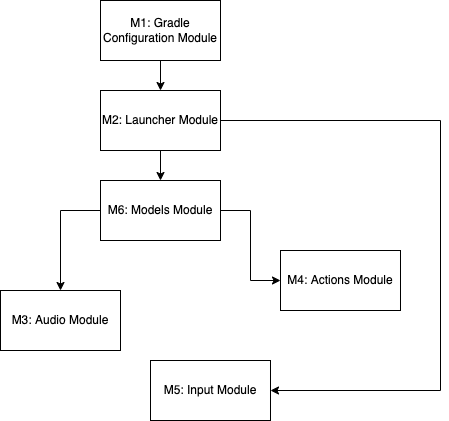
\includegraphics[width=0.7\textwidth]{Use Hierarchy Between Modules.png}
\caption{Use hierarchy among modules}
\label{FigUH}
\end{figure}

%\section*{References}

\bibliographystyle {plainnat}
\bibliography {MG}

\end{document}
